\documentclass[tikz]{standalone}

\usepackage{tikz}

\usepackage[T1]{fontenc}

\begin{document}
  \pagestyle{empty}

  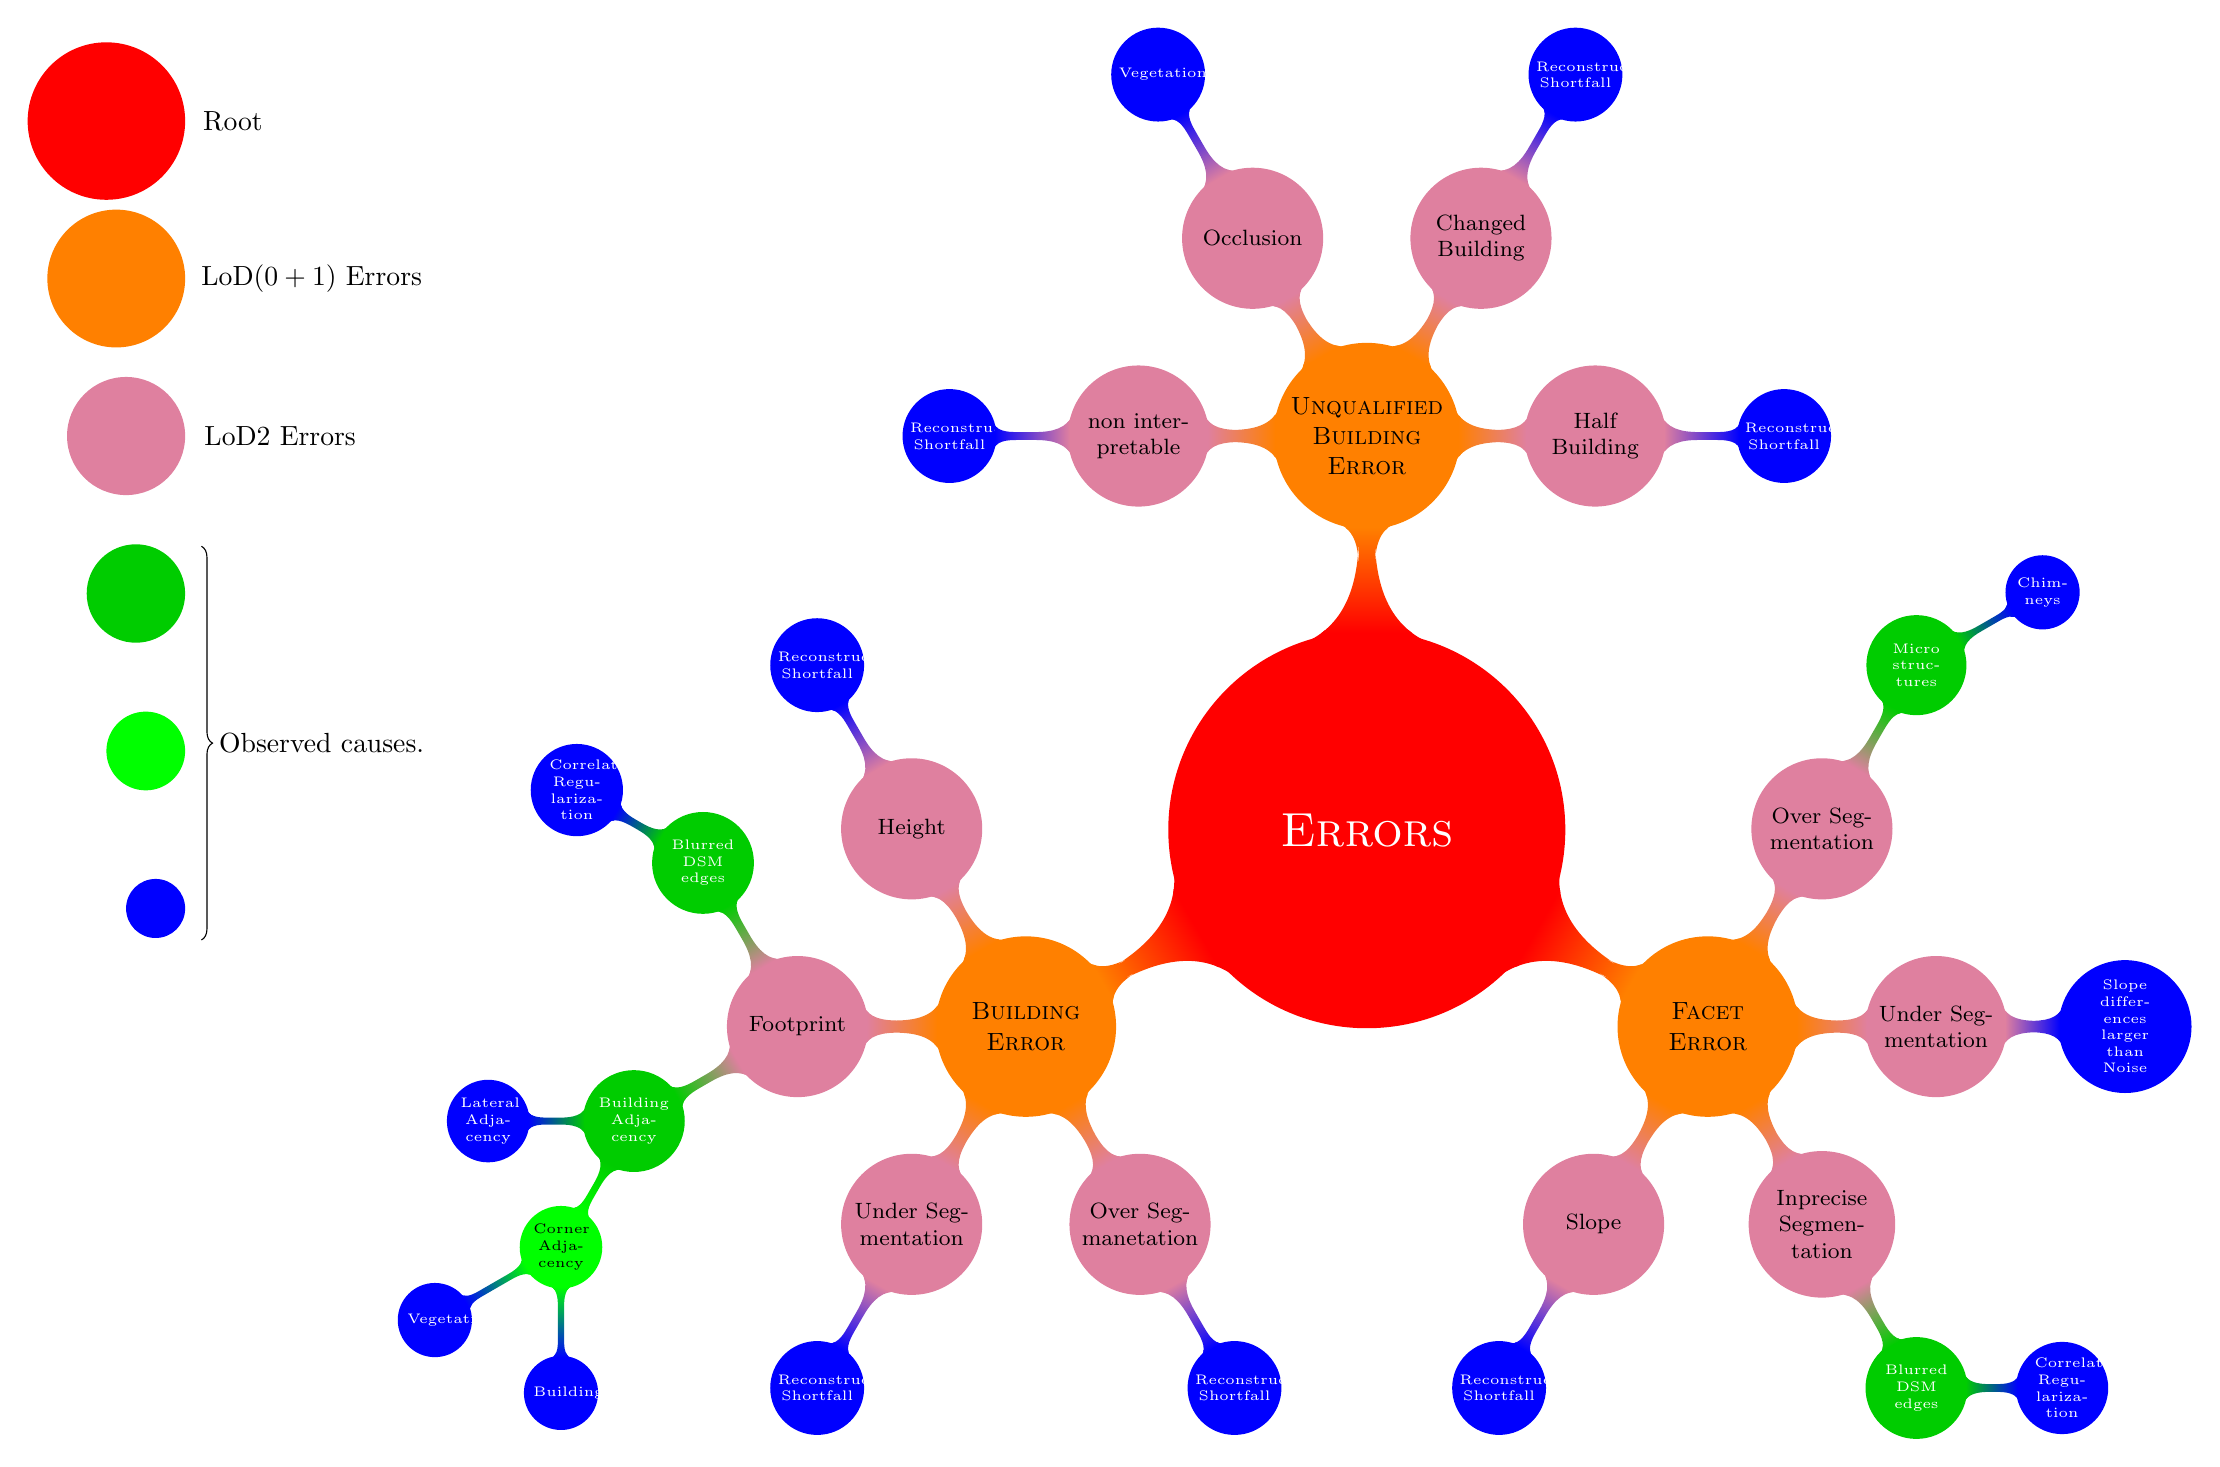
\begin{tikzpicture}
    \usetikzlibrary{mindmap, trees, decorations.pathreplacing}
    \node[circle, fill, color=red, minimum size=2cm, anchor=east] at (-15,9) (1) {};
    \node[text=black] at (-14.4, 9) {Root};
    \node[circle, fill, color=orange, minimum size=1.75cm, anchor=east] at (-15, 7) (2) {};
    \node[text=black] at (-13.4, 7) {LoD$(0 + 1)$ Errors};
    \node[circle, fill, color=purple!50, minimum size=1.5cm, anchor=east] at (-15, 5) (3) {};
    \node[text=black] at (-13.8, 5) {LoD$2$ Errors};
    \node[circle, fill, color=green!80!black, minimum size=1.25cm, anchor=east] at (-15, 3) (4) {};
    \node[circle, fill, color=green, minimum size=1cm, anchor=east] at (-15, 1) (5) {};
    \node[circle, fill, color=blue, minimum size=.75cm, anchor=east] at (-15, -1) (6) {};
    \draw[decorate,decoration={brace,amplitude=4pt}] (-14.8, 3.6) -- (-14.8, -1.4) node[midway, right, xshift=0.1cm, yshift=0pt]{Observed causes.};
    \path[mindmap, concept color=red, text=white]
      node[concept, minimum size=5cm]{\LARGE\textsc{Errors}}[clockwise from=0]
      child[concept color=orange, text=black, grow=90]
      {
        node[concept]{\textsc{Unqualified Building Error}}[clockwise from=0]
        child[concept color=purple!50, text=black, grow=0]
        {
          node[concept]{Half Building}[clockwise from=0]
          child[concept color=blue, text=white, grow=0]
          {
            node[concept]{Reconstruction Shortfall}
          }
        }
        child[concept color=purple!50, text=black, grow=60]
        {
          node[concept]{Changed Building}[clockwise from=0]
          child[concept color=blue, text=white, grow=60]
          {
            node[concept]{Reconstruction Shortfall}
          }
        }
        child[concept color=purple!50, text=black, grow=120]
        {
          node[concept]{Occlusion}
          child[concept color=blue, text=white, grow=120]
          {
            node[concept]{Vegetation}
          }
        }
        child[concept color=purple!50, text=black, grow=180]
        {
          node[concept]{non interpretable}
          child[concept color=blue, text=white, grow=180]
          {
            node[concept]{Reconstruction Shortfall}
          }
        }
      }
      child[concept color=orange, text=black, grow=330]
      {
        node[concept]{\textsc{Facet Error}}
        child[concept color=purple!50, text=black, grow=60]
        {
          node[concept]{Over Segmentation}
          child[concept color=green!80!black, text=white, grow=60]
          {
            node[concept]{Micro structures}
            child[concept color=blue, text=white, grow=30]
            {
              node[concept]{Chim-neys}
            }
          }
        }
        child[concept color=purple!50, text=black, grow=0]
        {
          node[concept]{Under Segmentation}
          child[concept color=blue, text=white, grow=0]
          {
            node[concept]{Slope differences larger than Noise}
          }
        }
        child[concept color=purple!50, text=black, grow=300]
        {
          node[concept]{Inprecise Segmentation}
          child[concept color=green!80!black, text=white, grow=300]
          {
            node[concept]{Blurred DSM edges}
            child[concept color=blue, text=white, grow=0]
            {
              node[concept]{Correlation Regularization}
            }
          }
        }
        child[concept color=purple!50, text=black, grow=240]
        {
          node[concept]{Slope}
          child[concept color=blue, text=white, grow=240]
          {
            node[concept]{Reconstruction Shortfall}
          }
        }
      }
      child[concept color=orange, text=black, grow=210]
      {
        node[concept]{\textsc{Building Error}}
        child[concept color=purple!50, text=black, grow=300]
        {
          node[concept]{Over Segmanetation}
          child[concept color=blue, text=white, grow=300]
          {
            node[concept]{Reconstruction Shortfall}
          }
        }
        child[concept color=purple!50, text=black, grow=240]
        {
          node[concept]{Under Segmentation}
          child[concept color=blue, text=white, grow=240]
          {
            node[concept]{Reconstruction Shortfall}
          }
        }
        child[concept color=purple!50, text=black, grow=180]
        {
          node[concept]{Footprint}
          child[concept color=green!80!black, text=white, grow=120]
          {
            node[concept]{Blurred DSM edges}
            child[concept color=blue, text=white, grow=150]
            {
              node[concept]{Correlation Regularization}
            }
          }
          child[concept color=green!80!black, text=white, grow=210]
          {
            node[concept]{Building Adjacency}
            child[concept color=green, text=black, grow=240]
            {
              node[concept]{Corner Adjacency}
              child[concept color=blue, text=white, grow=210]
              {
                node[concept]{Vegetation}
              }
              child[concept color=blue, text=white, grow=270]
              {
                node[concept]{Building}
              }
            }
            child[concept color=blue, text=white, grow=180]
            {
              node[concept]{Lateral Adjacency}
            }
          }
        }
        child[concept color=purple!50, text=black, grow=120]
        {
          node[concept]{Height}
          child[concept color=blue, text=white, grow=120]
          {
            node[concept]{Reconstruction Shortfall}
          }
        }
      };
  \end{tikzpicture}
\end{document}
